\section{Wstęp}
    \subsection{Założenia}
        \begin{itemize}
            \item Pomiar prądu rzędu $10\ nA$,
            \item Wykorzystanie ditheringu szumem Gaussowskim, 
            \item Wykorzystanie mikroprocesora STM32F103C8T6 z 12 bitowym ADC,
            \item Wykorzystanie wzmacniacza pomiarowego INA333.
        \end{itemize}
    \subsection{Schemat Blokowy}
    \begin{figure}[!ht]
        \centering
        \scalebox{1}{\begin{subfigure}{\textwidth}
    \hspace{0cm}
    \begin{tikzpicture}
        \draw
            (0, 0) node[op amp](amp1){}
            (0, -3) node[draw, rectangle, minimum width = 2cm, minimum height = 2cm, label = {[align = center]center:$V_{REF}$}](REF){}
            (3, -3) node[draw, rectangle, minimum width = 2cm, minimum height = 2cm, label = {[align = center]center:Noise \\Gen}]{}
            (5.5, -1) node[adder] (add) {}
            (7.5, -1) node[draw, rectangle, minimum width = 2cm, minimum height = 2cm, label = {[align = center]center:LPF}](LPF){}
            (12, -1) node[draw, rectangle, minimum width = 3cm, minimum height = 5cm, label = {[align = center]center:MCU}](MCU){}
            (12, -6) node[draw, rectangle, minimum width = 2cm, minimum height = 2cm, label = {[align = center]center:USB}](USB){}
            (7, -6) node[draw, rectangle, minimum width = 2cm, minimum height = 2cm, label = {[align = center]center:PSU}](PSU){}
            % (add.135) ++ (-1, 1) -- ++ (0.5, 0) -- (add)
            (add.225) ++ (-1.15, -1) -- ++ (0.5, 0) -- (add) 
            (add) -- ++ (1, 0)

            (amp1) ++ (0.3, -0.3) -- ++ (0, -1.7)
            (amp1.out) -- ++ (3.7, 0) -- (add)
            (amp1.+) -- ++ (-1, 0) to[/tikz/circuitikz/bipoles/length=20pt, R, l=$R_{meas}$] ++ (0, 1)
            (amp1.-) -- ++ (-1, 0) to[short, -o] ++ (0, 1) node[above]{$in-$}
            (amp1.+) ++ (-1, 0) to[short, -o] ++ (0, -1) node[below]{$in+$}
            (LPF) ++ (1, 0) -- ++ (2, 0) ++ (-0.75, 0) node[above]{$ADC_{in}$}
            (USB) ++ (0.5, 1) -- ++ (0, 1.5) ++ (0, -0.75) node[right]{$D-$}
            (USB) ++ (-0.5, 1) -- ++ (0, 1.5) ++ (0, -0.75) node[left]{$D+$}
            (PSU) ++ (1, 0) -- ++ (3, 0) ++ (-1, 0) node[above]{$+5\ V$}
            (PSU) ++ (-1, 0) to[short, -o] ++ (-1, 0) node[above]{$+3.3\ V$}
        ;
            % wzmacniacz pomiarowy, zrodlo ref, generacja szumu, sumator, MCU, USB, PSU, LPF
    \end{tikzpicture}
\end{subfigure}}
        \caption{Schemat blokowy układu do pomiaru natężenia prądu.}
        \label{sch:BD}
    \end{figure}
    \begin{figure}[!ht]
        \centering
        \scalebox{1}{    \begin{figure}[H]
        \centering
        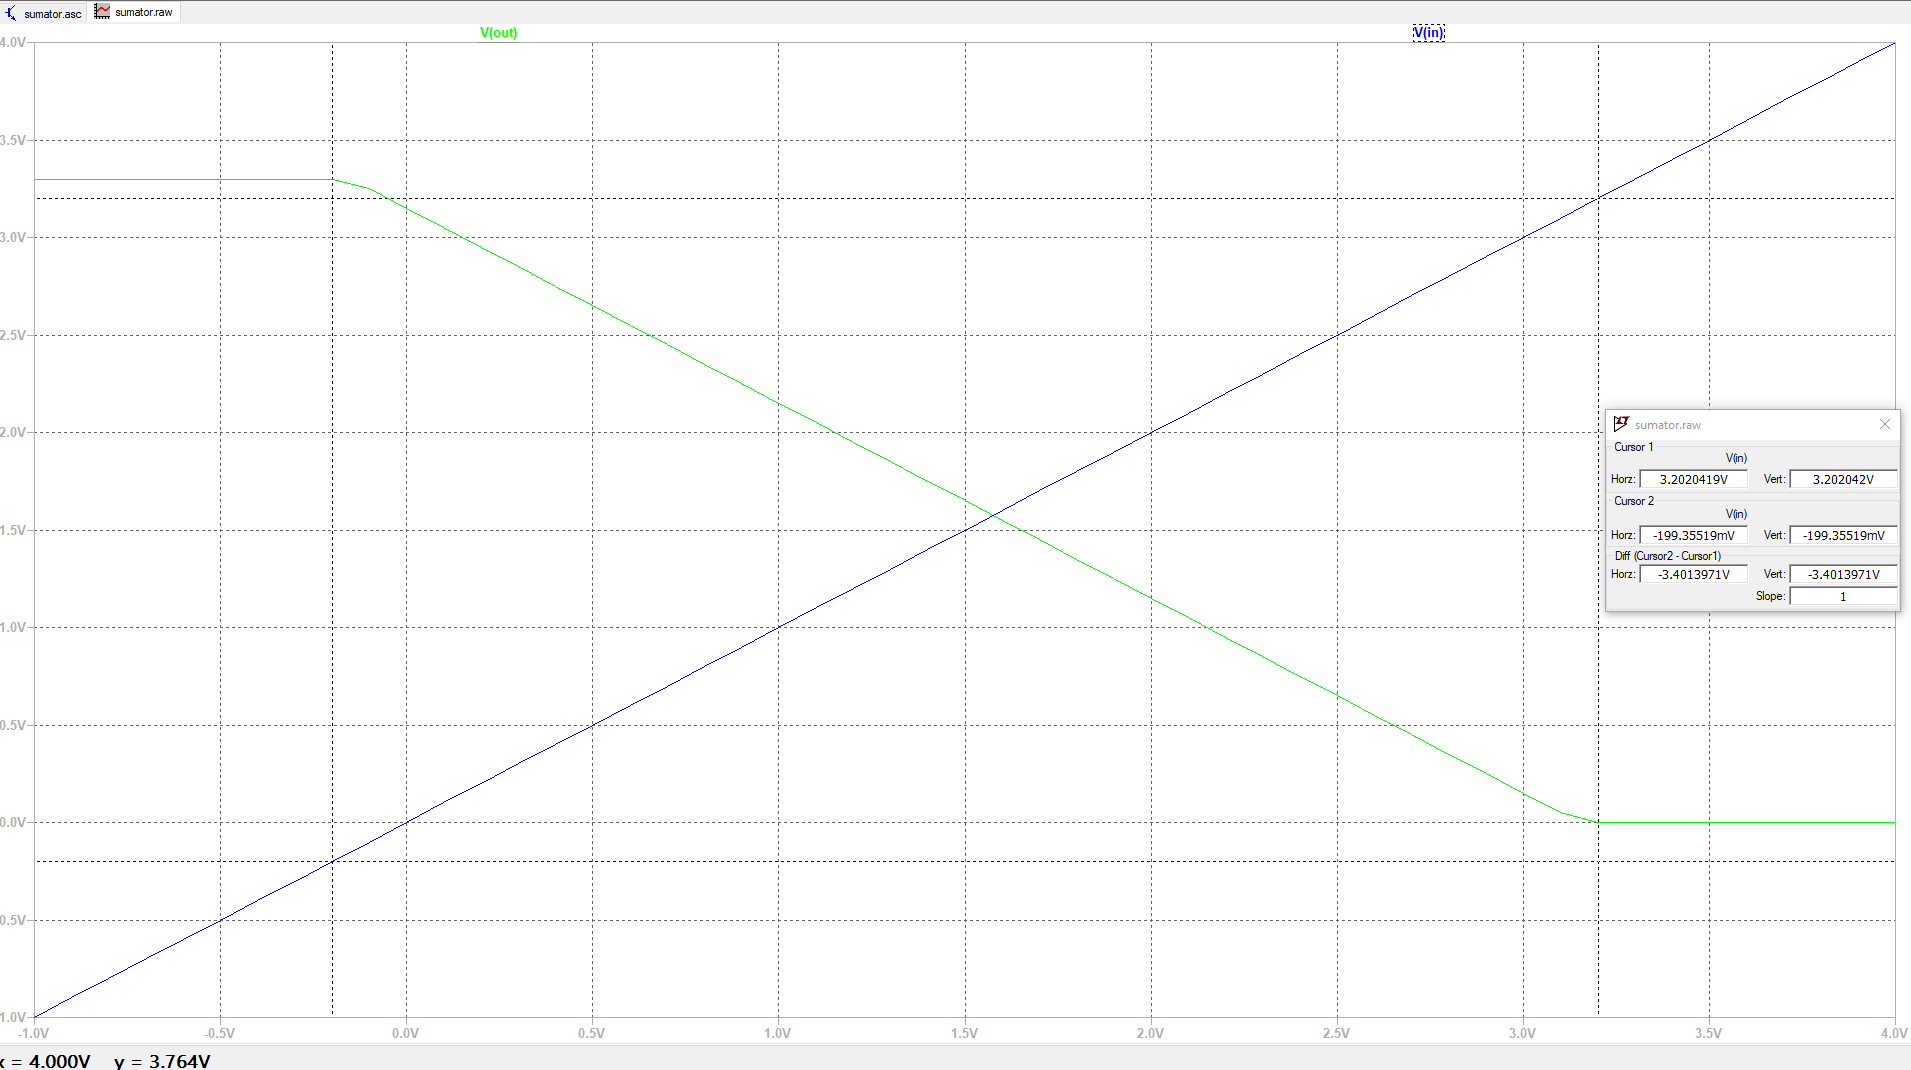
\includegraphics[width=1\linewidth]{images/sumator_dc.png}
        \caption{Symulacja dc układu sumującego, napięcia wyjściowego(Vout) od napięcia wejściowego (Vin)}
    \end{figure}}
        \caption{Układ sumacyjny dla dodania sygnału pomiarowego i szumu. }
        \label{sch:sumator}
    \end{figure}
    \begin{figure}[!ht]
        \centering
        \scalebox{1}{\begin{subfigure}{\textwidth}
    \hspace{4cm}
    \begin{tikzpicture}
    \draw
        (0, 0) node[draw, rectangle, minimum width = 3cm, minimum height = 3cm, label = {above:LT1117-3.3}](U1){}
        (U1.west) node[right=1mm] {IN}
        (U1.east) node[left=1mm] {OUT}
        (U1.south) node[above=1mm] {GND}
        (U1.south) node[ground]{}

        (U1.west) -- ++(-2,0) coordinate(IN)
        to[C, l=$C_{1}$, a=$10\ \mu$F] (IN |- U1.south) node[ground] {}
        (IN) to[short, -o] ++ (-1, 0) node[above]{$5V$}

        (U1.east) -- ++(2,0) coordinate(OUT)
        to[C, l=$C_{2}$, a=$100\ \mu$F] (OUT |- U1.south) node[ground] {}
        (OUT) to[short, -o] ++ (1, 0) node[above]{$3.3V$}

        ;
    \end{tikzpicture}
\end{subfigure}}
        \caption{Układ stabilizacji napięcia na 3.3V. }
        \label{sch:psu}
    \end{figure}